The influence of the Coriolis force on the currents of the ocean were first
noted by Hadley, Coriolis, and Ferrel. The the influence of these forces,
however, were considered too small and therefore didn't show in the theory of
the time \cite{Ekman1905}. Ekman's adviser Bjerknes was the first to indicate
the importance of the influence of the Earth's rotation in the theory of motions
of the ocean \cite{Ekman1905}. The true importance of the influence of the
Coriolis force was first noted by the Norwegian scientist Fridtjof Nansen
\cite{Beesley2008, Ekman1905}. Nansen designed a vessel, named the \emph{Fram},
with the intent of allowing it to freeze in the polar ice, and in 1898 Nansen
observed the drift of the \emph{Fram} from its original location. As the vessel
drifted Nansen noticed that the drift was always $20^\circ - 40^\circ$ to the
right of the wind current \cite{Beesley2008}.

\begin{wrapfigure}[9]{l}{0.5\textwidth}
  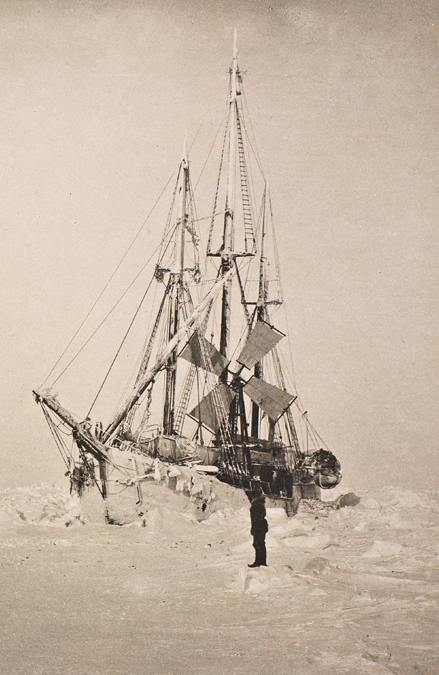
\includegraphics[scale=0.35]{Figures/Fram.jpg}
  \caption{The \emph{Fram} caught in ice in January 1895. Image courtesy of
  FramMuseum.no}
  \label{fig:Fram}
\end{wrapfigure}
In 1905 Ekman \cite{Ekman1905} took the observations made by Nansen and developed
what is considered to be the origin of modern theories for wind-driven ocean
circulation and their effects on ocean currents \cite{Price1987}. According to
Ekman theory momentum from the wind is transferred at the surface of the ocean
to the water, as it blows across the ocean surface, via wind stress. Then the
Earth's rotation imparts a Coriolis acceleration on the moving water which
causes a deflection of the transport to the right of the surface wind stress in
the Northern Hemisphere and to the left of the surface wind stress in the
Southern Hemisphere \cite{Beesley2008}.

Rossby in his 1936 paper \cite{Rossby1936} introduced a force which he says had
been ``completely disregarded by theoretical investigators although its
existence has been admitted implicitly by practically everyone who has approached
physical oceanography from the descriptive side.'' The force that Rossby
introduced was the frictional force resulting from large-scale horizontal
mixing. According to Rossby, ``The introduction of this force permits us to see
how motion generated in the surface layers may be diffused and finally
dissipated without recourse to doubtful frictional forces at the bottom of the
ocean.'' Additionally, a significant contribution of Rossby was that he noticed
one could represent the Coriolis force by \cite{James2009}
\begin{equation}
  f = f_0 + \beta\, y,
  \label{eqn:CoriolisParameterization}
\end{equation}
where $f$ is the Coriolis parameter, $f_0$ is the reference Coriolis parameter,
$\beta$ is the $\beta$-plane parameter, and $y$ is the $y$-coordinate (oriented
northward).

Then Sverdrup introduced the idea of a variable \emph{Coriolis parameter}
\cite{Fox-Kemper2003}. By allowing for the variation of the Coriolis parameter
in the north-south direction Sverdrup \cite{Sverdrup1947} introduced, for the
first time, a north-south asymmetry of the problem domain. The term he
introduced, $\nabla \cdot (\mathbf{x} \psi)$ is known as the $\beta$-term
because of the typical notation for the derivative of the Coriolis parameter
\cite{Fox-Kemper2003}. This asymmetry in the north-south direction accounted for
the heretofore unexplained equatorial countercurrents.

Ekman's theory explains the deflection of ocean currents from the direction of
the wind stress and Sverdrup's allowed for an asymmetry in the north-south
direction, thereby resolving the matter of equatorial countercurrents.  The
combination of the two, however, was still not able to explain the existence of
strong western boundary currents \cite{Fox-Kemper2003}.  Next, Stommel
\cite{Stommel1948} noticed that taking the gradient of the Coriolis term
introduced an asymmetry in not only the north-south direction, but also in the
east-west direction. This new term, $\dfrac{\partial \psi}{\partial x}$, which
involves the streamfunction $\psi$ introduces an asymmetry in the east-west
direction. This can be seen by substituting $-x$ for $x$: clearly the sign of
the $\beta$-term changes. This $\beta$-term is a convective term resulting from
the rotation of the Earth. The model developed by Stommel was a simple model
which included the $\beta$-term, a bottom friction term ($-\delta_S \nabla^2
\psi$), and a wind stress forcing term ($F$).  The resultant equation is
\cite{Fox-Kemper2003,Stommel1948,Vallis06}
\begin{equation}
  \frac{\partial \psi}{\partial x} = F - \delta_S \nabla^2 \psi.
  \label{eqn:StommelModel}
\end{equation}
Stommel noted that without the $\beta$-term the solution would be
symmetric in the east-west direction and therefore no western boundary current
would exist \cite{Stommel1948}.

Soon after Stommel's 1948 paper, Munk \cite{Munk1950} published a paper on the
westward intensification of ocean currents. In his paper, Munk explains that
``[i]n Ekman's and Stommel's model the ocean is assumed homogeneous, a case
which the currents extend to the very bottom.'' Munk points out that this is
``in contrast with observations'' and resulted in ``very difficult'' analysis
for Ekman while Stommel was forced ``to resort to a rather arbitrary frictional
force along the bottom.'' To address this Munk introduces lateral friction with
a constant viscosity. Thus, the Munk problem is
\cite{Fox-Kemper2003,Munk1950,Vallis06}
\begin{equation}
  \frac{\partial \psi}{\partial x} = \delta_M^3\, \Delta^2 \psi + F,
  \label{eqn:MunkProblem}
\end{equation}
where $\delta_m$ is the Munk scale. In addition to the introduction of lateral
viscosity, the Munk problem introduced a fourth-order operator (the biharmonic
operator), which required an extra boundary condition.  In Munk's 1950
paper \cite{Munk1950}, he used the same boundary conditions that we will
consider, i.e. $\dfrac{\partial \psi}{\partial \mathbf{n}} = 0$, where
$\mathbf{n}$ is the outward unit normal vector.

In 1948 Charney \cite{Charney1948} introduced a method by which he ``filtered out
the noise'' from meteorological equations. By filtering out the so-called noise
of the meteorological equations Charney was able to greatly simplify the
equations of motion for the ocean and atmosphere, thus allowing for numerical
weather prediction, which seemed to previously suffer from unsurmountable
complexities. This method of filtering is known as the quasi-geostrophic
approximation, and relies on the assumption that the Rossby number
\begin{equation}
  Ro = \frac{U}{f\, L},
  \label{eqn:RossbyNumber}
\end{equation}
where $U,\, L$ are the characteristic velocity and length, respectively, is
much much smaller than one. Later in his 1949 paper \cite{Charney1949} Charney
introduced a method ``for reducing the three-dimensional forecast problem to a
two-dimensional one.'' It is the equations Charney introduced in this 1949 paper
that has now come to be called the quasi-geostrophic equations and is the main
focus of this thesis.
